
\documentclass[11pt,a4paper]{article}

% Preamble
\usepackage[utf8]{inputenc}
\usepackage[T1]{fontenc}
\usepackage{geometry}
\geometry{a4paper, margin=1in}
\usepackage{amsmath, amssymb, amsfonts}
\usepackage{graphicx}
\usepackage{booktabs}
\usepackage{hyperref}
\usepackage{caption}
\usepackage{float}
\usepackage{xcolor}
\usepackage{array}
\usepackage{float}

% Formatting
\hypersetup{
    colorlinks=true,
    linkcolor=blue,
    filecolor=magenta,      
    urlcolor=cyan,
}

\title{
    \vspace{-2cm}
    % \includegraphics[width=0.4\textwidth]{kth_logo.png} \hfill \text{KTH Formula Student} \\
    \vspace{2cm}
    \textbf{Interior Permanent Magnet Motor Design} \\
    \large Design to Improve the Formula Student Team Car's Performance
}
\author{IPM Design Team}
\date{\today}

\begin{document}

\maketitle
\newpage

\tableofcontents
\newpage

\section{Background: Current Motor and Inverter Analysis}
The KTH Formula Student team has an already working racing car that has been used in different competitions. This section analyses both Motor and Inverter in order to define a baseline for the new design, focusing on reducing the current motor's limitations and improving the overall performance, tailored to the needs of the team. 
\subsection{Motor}
The team currently utilizes four \textbf{DD5-14-10-POW-18600-B5} motors to power their vehicle. This vehicle is used in different competitions with different terrains. From a flat long track where speed is needed, to auto-cross scenarios where torque is critical. Due to that reason, the car should be able to perform in a variety of conditions. From datasheets and pictures, the following characteristics were identified:
\\\textbf{Winding Configuration:} 86 wire ends, indicating a total number of turns per tooth of 43. See Figure \ref{fig:stator_stator_rotor} (left).
\\\textbf{Slot Number:} 12 slots, which gives a slot per pole ratio of 1.2 (12 slots / 10 poles), indicating a non-integer slot winding configuration. See Figure \ref{fig:stator_stator_rotor} (center).
\\\textbf{Rotor Topology:} Interior permanent magnet (IPM) topology. See in Figure \ref{fig:stator_stator_rotor} (right).
\\\textbf{Inductance Profile:} According to the datasheet, the baseline motor exhibits saliency where $L_d = 0.24$ mH and $L_q = 0.12$ mH ($L_q < L_d$).\\

\begin{figure}[H]
    \centering
    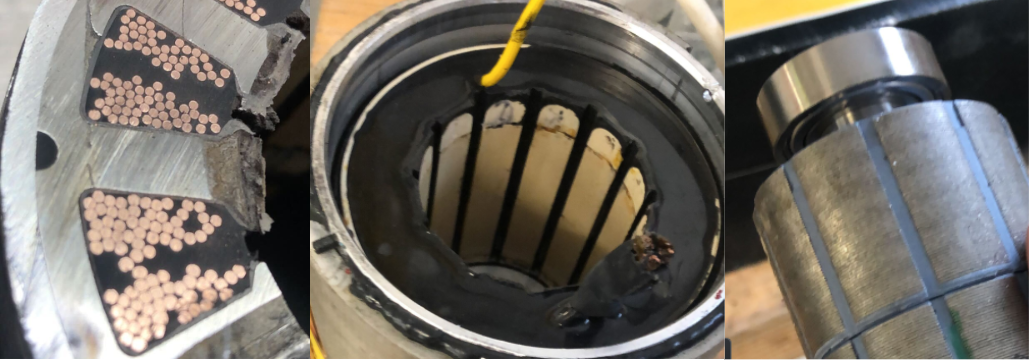
\includegraphics[width=0.7\linewidth]{figures/stator_stator_rotor.png}
    \caption{Left: Traversal cut of the stator. Center: Stator. Right: Rotor.}
    \label{fig:stator_stator_rotor}
\end{figure}
The Fig. \ref{fig:side_technical_drawing} and Fig. \ref{fig:front_technical_drawing} had been extracted from the datasheet, and we can see how the winding heads space have to be considered for the stack length calculation; meaning that the true stack length limit is 110mm - winding heads = 110mm - 24.8mm = \textbf{85.2 mm}. For the diameter, we can keep the \textbf{80 mm} limit.
This is a constraint that has to be considered in the new mechanical design.
Also, its worth it mentioning that the same motor/inverter configuration is used for the front and rear wheels, meaning that the new design should be compatible with both axles. A further discussion on this will be made in this document.
\begin{figure}[H]
    \centering
    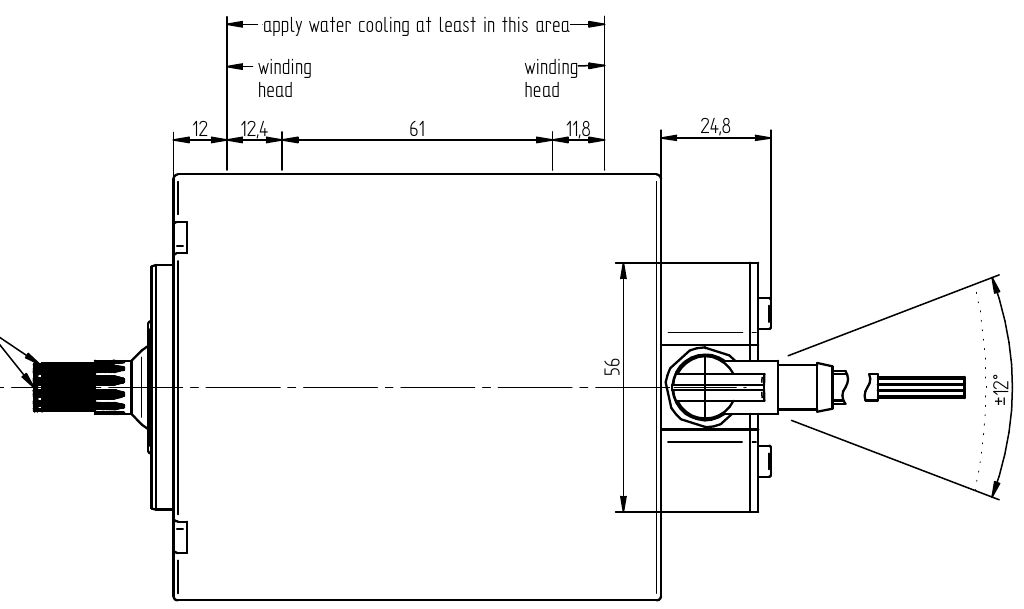
\includegraphics[width=0.75\linewidth]{figures/side_technical_drawing.png}
    \caption{Side view of the current motor.}
    \label{fig:side_technical_drawing}
\end{figure}
\begin{figure}[H]
    \centering
    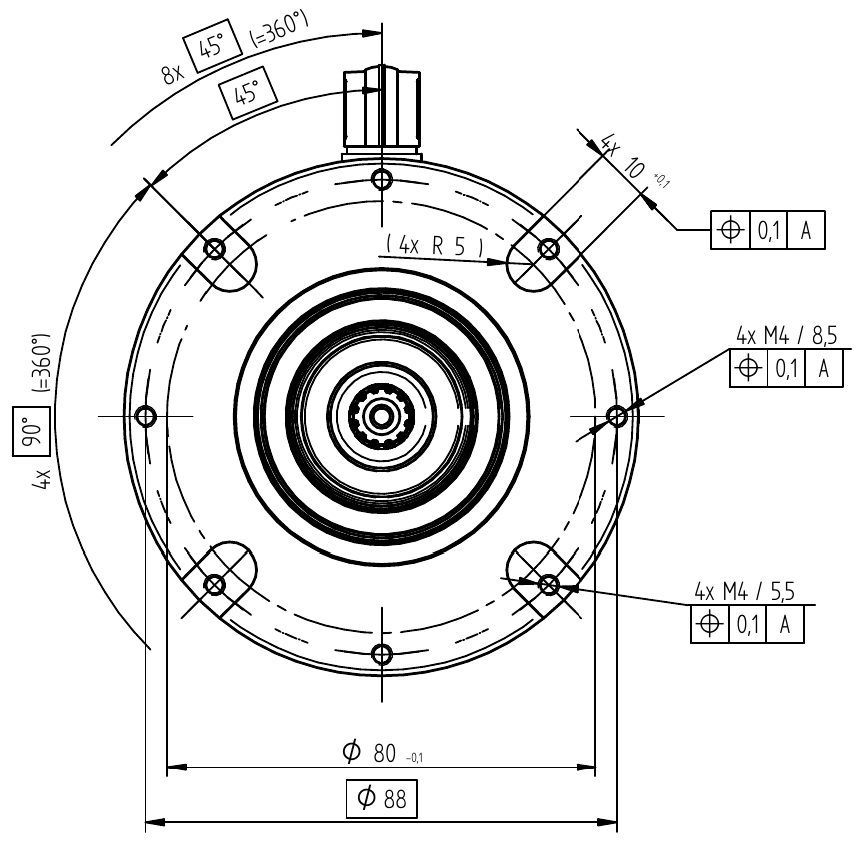
\includegraphics[width=0.70\linewidth]{figures/front_technical_drawing.png}
    \caption{Front view of the current motor.}
    \label{fig:front_technical_drawing}
\end{figure}
Moreover, each motor is connected to a fixed gearbox with a 14:1 ratio, which will be kept for the new design. Thus any further speed calculation has to consider that the motor rotates 14 times faster than the wheel. Also, note from Fig. \ref{fig:power_and_torque_current_motor} how the current motor can operate in field-weakening mode only from 16000 rpm up to the 20000 rpm limit, meaning the machine has a"Flux-weakening ratio" of 1.52 (20,000 rpm / 13,200 rpm). We will briefly see in section \ref{sec:Inverter} that the KW26-S5-FSE-4Q inverter only allows for a max. speed of 14,000 rpm, thus leaving a real flux-weakening ratio of only 1.1 (14,400 rpm / 13,200 rpm). For the new design, we aim to increase this ratio.
\begin{figure}[H]
    \centering
    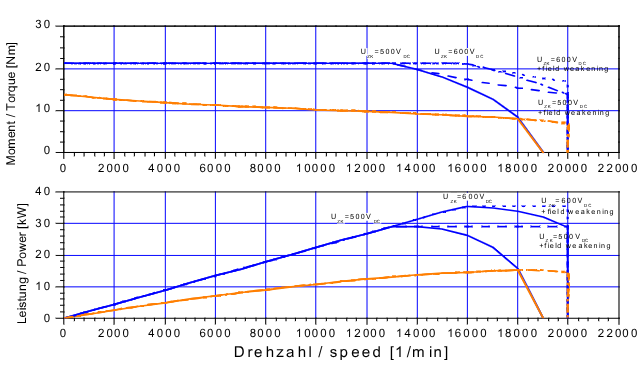
\includegraphics[width=0.75\linewidth]{figures/power_and_torque_current_motor.png}
    \caption{From datasheet: Power and Torque vs Speed for the current motor.}
    \label{fig:power_and_torque_current_motor}
\end{figure}
\subsection{Inverter}
\label{sec:Inverter}
The inverter used to drive this motor is the \textbf{KW26-S5-FSE-4Q}. This inverter consists of 4 independent channels.
Notice how the inverter is a bottleneck in this configuration, since the 1200 Hz limit gives a 14,400 rpm for a 10-pole machine. This means that the motor enters field-weakening mode only on the last 10\% range of operation.
%For our first design iteration, we will allow ourselves to think of an ideal inverter, focusing entirely on the motor design. In a later stage, we will consider the inverter limitations and even consider the acquisition of a new inverter if needed.

The following table summarizes the previously analyzed motor parameters and the datasheet values.
\begin{table}[H]
\centering
\caption{Current motor parameters (DD5-14-10-POW)}
\label{tab:current_motor_data}
\begin{tabular}{p{4cm} l p{6.8cm}}
\hline
\textit{Parameter} & \textit{Symbol} & \textit{Value}\\ \hline
\textbf{Pole Number} & $P$ & 10 \\
\textbf{Slot Number} & $S$ & 12 \\
\textbf{Line Voltage} & $V_{line}$ & 540 V\\
\textbf{Nominal Power} & $P_{n}$ & 12.3 kW \\
\textbf{Peak Power} & $P_{max}$ & 28 kW \\
%\textbf{Nominal Torque} & $T_{nom}$ & 10 Nm \\
\textbf{Nominal Torque} & $M_{n}$ & 9.8 Nm \\
%\textbf{Peak Torque} & $M_{clip}$ & 18 Nm \\
\textbf{Nominal Speed} & $N_{n}$ & 12,000 rpm \\
\textbf{Max.Speed} & $N_{max}$ & 14,400 rpm \\
\textbf{Characteristic Speed Point} & $N_{char}$ & 13,200 rpm \\
\textbf{Gear Ratio} & $G$ & 14:1 \\
\textbf{Stack Length} & $L$ & 85.2 mm \\
\textbf{Diameter} & $D$ & 80 mm \\
\textbf{Aspect ratio} & $L/D$ & 1.065 \\
\textbf{Flux-weakening Ratio (inverter constrained)} & $N_m/N_c$ & 1.1 \\
\textbf{Rotor Topology} & --- & Interior Permanent Magnet \\ \hline
\end{tabular}
\end{table}

\section{Part A: Framework Definition and Requirements}
In the following sections, we will define the initial values and limitations that will guide the design of the new motor. We will start by defining the boundary requirements, which are the constraints that the new design should respect.
\subsection{Boundary Requirements}
The following table summarizes those design boundaries, which are constrained by the inverter properties, mechanical enclosure and the Formula Team itself. The new design should stick to these requirements, and any design deviation should be justified.
\begin{table}[H]
\centering
\caption{Boundary requirements for the new propulsion motor design.}
\label{tab:propulsion_motor_requirements}
\begin{tabular}{@{}p{0.62\linewidth}p{0.30\linewidth}@{}}
\toprule
\multicolumn{2}{@{}l@{}}{\textbf{General requirements}} \\
\midrule
Max dimensions including cooling (outer diameter $\times$ length) & 120 mm $\times$ 110 mm \\
Hub compatible & Must \\
Motor topology & Radial in-runner (rotor inside the stator) \\
Weight & $\leq$ 2800 g \\
Power density (mass) & $\geq$ 10 kW/kg \\
IP protection & IP65 \\
\addlinespace
\multicolumn{2}{@{}l@{}}{\textbf{Mechanical requirements}} \\
\midrule
Peak torque (for 5 s) & 21.5 Nm \\
Maximum speed & 20000 rpm \\
Nominal torque & 9.8 Nm \\
Nominal speed & 12000 rpm \\
\addlinespace
\multicolumn{2}{@{}l@{}}{\textbf{Electrical requirements}} \\
\midrule
Operating Voltage ($V_{LL, RMS}$) & 235 V to 420 V \\
%Source Voltage (input for inverter) & 515 $V_{DC}$ \\
%Machine Voltage Input ($V_{LL, RMS}$) & 334 $V_{AC}$ \\
%Machine Voltage Input ($V_{LN, RMS}$) &  202 $V_{AC}$ \\
Peak power & 28 kW \\
Average power & 12 kW \\
Three-phase cable diameter & 11 mm $\pm$ 0.5 mm \\
\addlinespace
\multicolumn{2}{@{}l@{}}{\textbf{Sensor requirements}} \\
\midrule
Rotor position & Must \\
Stator temperature & Must \\
Rotor temperature & Preferred \\
\addlinespace
\multicolumn{2}{@{}l@{}}{\textbf{Cooling requirements}} \\
\midrule
Coolant & Liquid or air \\
Cooling circuit & External or internal \\
\addlinespace
\multicolumn{2}{@{}l@{}}{\textbf{Compatibility}} \\
\midrule
Rotary encoder & ECI1118, P-type \\
Output spline & DIN 5480 - W11x0,8x30$^\circ$x30x12x7h \\
\bottomrule
\end{tabular}
\end{table}
\subsection{First Design Objectives}
Now, we will define our design target parameters, using the current motor parameters (Table~\ref{tab:current_motor_data}) as a starting point, and aiming to respect the boundary requirements (Table~\ref{tab:propulsion_motor_requirements}).
Similarly to the old design, we will use permanent magnets due to their high power density, taking into consideration the thermal limits. We will avoid surface permanent magnets (SPM) because the use of glue introduces mechanical challenges. On the other hand, the interior permanent magnet (IPM) topology allows a more robust mechanical design and the possibility to have a higher saliency ratio ($L_q/L_d$), Moreover, \textbf{We aim to invert the saliency in order to make $L_q$ > $L_d$}; This new topology will allow a wider field-weakening operation mode, increasing the knee point we saw in \ref{fig:power_and_torque_current_motor}. which is beneficial for field-weakening operation. \\
\subsubsection{Rotor Design}
To translate the performance requirements into initial physical dimensions, we utilize two formulas.
\subsubsection*{Formula 1: Esson's Rule}
This simple formula lets us estimate the mechanical power of a machine based on its physical dimensions and magnetic properties. Notice how the torque does not depend on the number of poles.
$$P_{mech} = \frac{\pi^2}{120}\omega_r[rpm](D_{is}^2l_e)B_{g,1}\,K_{s,1}\,\eta_{gap}\,cos(\phi_{gap})$$
Here we define the \textbf{"Magnetic shear stress"} term as:
$$\sigma_m = \frac{B_g,1\,K_{s,1}}{2}\;[N/m^2]$$
And if we neglect the air gap, we get \cite{??}:
$$\tau = 2V_{rotor}\sigma_m\eta_{gap}cos(\phi_{gap})$$
Simplified:
\begin{equation}
\label{eq:essons_rule}
T = \sigma_m \cdot D_{is}^2 L
\end{equation}
Now we have to select the magnetic shear stress value. Permanent magnet machines which do not have a rotor current disadvantage typically fall in the range from 40,000 to 60,000 $N/m^2$. As an upper limit, liquid-cooled machines having a shear stress of up to 100,000 $N/m^2$ have been reported \cite{Lipo2017}.
Therefore, we target an initial value of \textbf{$\sigma_m = 50,000$ N/m$^2$}. We can allow this design choice thanks to the cooling loop, and the fact that transient nature of racing allows will have transient peaks in loading, compared to continuous-duty industrial applications.
We still have two degrees of freedom, the rotor diameter and the stack length. We know that the aspect ratio ($L/D$) typically falls in the range of 1.0 to 2.0. A large aspect ratio is beneficial for weight (and thus cost) reduction, but the stator current density increases, making harder to cool down the machine. On the other hand, a smaller aspect ratio has a poorer performance in terms of torque due to the end-winding leakage inductance affecting the available torque \cite{LucaLecture6}.
For now, we assume we will have the same aspect ratio $L/D = 1.065$ as in the previous motor (Tab. \ref{tab:current_motor_data}). Then, we solve Eq. \ref{eq:essons_rule} for $L$ and $D$:
\begin{align*}
L &= 1.065 D \\
T &= \sigma_m D^3 1.065 \\
D &= \sqrt[3]{\frac{T}{\sigma_m \cdot 1.065}} = \sqrt[3]{\frac{9.8\,Nm}{50,000\cdot 1.065}} = 56.88\,\text{mm} \\
L &= 1.065 D = 60.58\,\text{mm}
\end{align*}
This results in a stack length of 60.58 mm, which is well within the ?? limit. This gives us an idea that the new design is feasible, and even more, it can even be smaller in size than the current one. Nevertheless, it is important to keep in mind during the design that we are assuming a $\sigma_m$ target of 50,000 $N/m^2$, which depends on the magnet material selection and a a relatively high magnetic flux linkage.
\subsubsection*{Formula 2: The $D^3L$ Output Coefficient}
% TODO
\subsubsection*{Pole Number}
For the number of poles, we will use 10 as the previous motor, because it is already optimized for the 1200 Hz inverter limit at 12,000 rpm.
The corresponding electrical frequency is
\begin{equation}
    f_{el} = \frac{pole\;pairs\cdot N_n}{60} = \frac{10/2 \cdot 12,000}{60} = 1000\,\text{Hz}
\end{equation}

\subsubsection{Stator Design}
We will keep the same number of slots (12) as the current motor, %TODO: fill with a good reason. I think the non-integer slot winding configuration is beneficial for reducing cogging torque.
Also, we will consider increasing the winding turns from the current 43, to allow for higher magnetic flux linkage and thus letting the back-EMF reach the DC bus voltage limit at a lower speed, while reducing $I^2R$ losses for the nominal speed. and enabling us to use the motor in the field-weakening mode for a wider speed range.
\subsubsection*{Theoretical Foundation of Base Speed}
The point where torque begins to fall is defined as the Base Speed ($\omega_{base}$), occurring when the motor's internal Back-Electromotive Force (Back-EMF) reaches the maximum voltage available from the inverter. This relationship is governed by:

\begin{equation}
\omega_{m,base} \approx \frac{V_{\text{phase,peak,max}}}{p\,\Psi_m}
\end{equation}

Where $V_{\text{phase,peak,max}}$ is the maximum achievable \emph{phase} fundamental peak voltage, $p$ is the number of pole pairs, and $\Psi_m$ is the permanent magnet flux linkage. 

The currently used AMK invervrter considers a maximum continuous modulation index of $M_i=0.917$, which limits the maximum fundamental phase voltage to:
\begin{equation}
    V_{\text{phase,peak,max}} = M_i \frac{V_{DC}}{\sqrt{3}} \approx 0.917 \times \frac{515}{\sqrt{3}} \approx 273\,\text{V}
\end{equation}
To trigger the torque droop at an earlier speed, we must increase $\Psi_m$ (e.g., by increasing stator turns or selecting higher remanence magnets), thereby reducing $\omega_{m,base}$.

For example, targeting $n_{base}=10{,}000\,\text{rpm}$ with $p=5$ gives a mechanical speed of $\omega_{m,base}\approx 1047\,\text{rad/s}$. Using the available $V_{\text{phase,peak,max}}\approx 273\,\text{V}$ yields a required order-of-magnitude flux linkage of:
\begin{equation}
    \Psi_m \approx \frac{V_{\text{phase,peak,max}}}{p\,\omega_{m,base}} \approx \frac{273}{5 \cdot 1047} \approx 0.0528\,\text{Wb}
\end{equation}
\subsubsection*{Magnet Material Selection}
TBD
The following table summarizes the first design objectives.
\begin{table}[H]
\centering
\caption{New Design Objectives}
\label{tab:motor_design_data}
\begin{tabular}{p{3.1cm} l l p{9cm}}
\hline
\textit{Parameter} & \textit{Symbol} & \textit{Value} & \textit{Engineering Justification} \\ \hline
\textbf{Pole Number} & $P$ & 10 & Sized to maximize the AMK RACING KIT inverter capacity (26 kVA/channel) while respecting the inverter DC bus ceiling (515 V). \\
\textbf{Length x Diameter} & $L \times D$ & 21.9 mm x 80 mm & jajjaj\\
\textbf{Line Voltage} & $V_{line}$ & 515 V & It is under the 540V nominal value of the inverter. \\
\textbf{Target Nominal Power} & $P_{nom}$ & 10 kW & \textbf{*} This value sits below the current motor rating (12.4 kW) and requirement (12 kW), but still meets the application requirements. This reduction is justified by the expectation that the operating conditions doesnt need full power (eg. The team mentioned using either 30\% or 80\% of the motor's full capacity)\\
\textbf{Target Peak Power} & $P_{peak}$ & 28 kW & Sized to maximize the AMK RACING KIT inverter capacity (26 kVA/channel) while respecting the inverter DC bus ceiling (515 V). \\
\textbf{Target Nominal Torque} & $T_{nom}$ & 7 Nm & \textbf{*} It is below the current motor rating (10 Nm) and requirement (9.8 Nm). This deviation is acceptable because the motors are used at 30\% of its capacity for the front wheels.\\
\textbf{Clipped Peak Torque} & $M_{clip}$ & 18 Nm & Software clip to ensure mechanical reliability of the transmission and manage thermal saturation. \\
\textbf{Target Max Speed} & $n_{max}$ & 12,000 rpm & Constrained by the 1200 Hz inverter limit; provides a 20\% safety margin (1000 Hz at 12,000 rpm for 10 poles). \\
\textbf{Target Nominal Speed*} & $n_{nom}$ & 10,000 rpm & \textbf{*} This value is under the 12,000 rpm constraint defined earlier. The reason for this deviation is that we are going to optimize for Field Weakening Mode.\\
\textbf{Gear Ratio} & $G$ & 14:1 & Fixed by the current powertrain package to optimize acceleration out of tight autocross corners. \\
\textbf{Rotor Topology} & --- & IPM & Selected to achieve $L_q > L_d$, enabling reluctance torque to hit the 18 Nm target under the 107 A inverter limit. \\ \hline
\end{tabular}
\end{table}

\section{Phase 2: Analytical Design and Rotor Parameterization}

To establish a robust first-principle model prior to Finite Element Analysis (FEA) in COMSOL, the analytical procedure proposed by Di Gerlando and Ricca is implemented. This approach defines the critical V-shape geometry based on structural constraints and evaluates the cross-coupling magnetic saturation.

For traceability, Table~\ref{tab:comsol_param_set} summarizes the \textbf{current} geometry and operating-point parameters pushed from MATLAB into the COMSOL model.

\begin{table}[H]
\centering
\caption{COMSOL parameter set used by the MATLAB automation} % (single source: \texttt{MATLAB\_to\_COMSOL\_Interface.m}).}
\label{tab:comsol_param_set}
\begin{tabular}{@{}p{0.44\linewidth}p{0.18\linewidth}p{0.30\linewidth}@{}}
\toprule
\textbf{Parameter} & \textbf{Symbol} & \textbf{Value} \\
\midrule
Number of poles & $N_p$ & 10 \\
Number of slots & $N_s$ & 12 \\
Rotor diameter & $d_r$ & 80 mm \\
Stator diameter & $d_{st}$ & 100 mm \\
Airgap & $g$ & 0.7 mm \\
Stack length (sized) & $L$ & from Essen's rule + winding head \\
Inverter current limit & $I_{pk}$ & 107 A (phase peak) \\
Speed (operating cap) & $n_{max}$ & 12,000 rpm \\
Magnet width (slab) & $w_m$ & 14 mm \\
Magnet thickness & $t_m$ & 3.5 mm \\
V-angle & $\alpha_v$ & 130$^\circ$ \\
Outer bridge thickness & $b_t$ & 1.0 mm \\
\bottomrule
\end{tabular}
\end{table}

\subsection{Rotor Bridge Sizing and Structural Integrity}
The structural integrity of the IPM rotor is heavily dependent on the sizing of the inner ($w_{ib}$) and outer ($w_{ob}$) iron bridges. In this project the real operating cap is $n_{max}=12{,}000\,\text{rpm}$ (inverter/electrical frequency constraint), and the bridge stress check is performed at this speed.
Electromagnetically, these bridges must be as thin as possible to minimize permanent magnet (PM) flux leakage. Mechanically, they must withstand the centrifugal forces exerted by the PM segments and the iron pole shoe.

Following the analytical model, the outer bridge is fixed to a minimum practical manufacturing thickness. In the current COMSOL iteration this is set to $b_t=1.0\,\text{mm}$, while the inner bridge is sized to sustain the primary centrifugal load.

The maximum angular velocity for a mechanical speed $n_{max}$ is:
\begin{equation}
    \Omega_{max} = \frac{2\pi n_{max}}{60}
\end{equation}
For $n_{max}=12{,}000\,\text{rpm}$, $\Omega_{max}\approx 1257\,\text{rad/s}$.

The specific maximum centrifugal force ($f_{max}$) is calculated based on the mass of the pole shoe and magnets ($m_{1p}$) at average radius ($R_{av}$):

\begin{equation}
    f_{max} = m_{1p} \cdot R_{av} \cdot \Omega_{max}^2
\end{equation}

As a first-order estimate, the magnet contribution to $m_{1p}$ can be computed from the present geometry (two magnets per pole) as:
\begin{equation}
    m_{pm,1p} \approx 2\,\rho_{pm}\,w_m\,t_m\,L
\end{equation}
where $\rho_{pm}$ is the magnet density, $w_m=14\,\text{mm}$, $t_m=3.5\,\text{mm}$, and $L$ is the active stack length.

The stress on the inner bridge is then evaluated against the lamination yield strength ($\sigma_{y,lam}$) using a stress concentration factor ($K_t$):
\begin{equation}
    \sigma_{ib} = K_t \cdot \frac{f_{max}}{w_{ib} \cdot k_{st}} \leq \sigma_{y,lam}
\end{equation}

\subsection{V-Shape Parametric Definition}
With the 10-pole arrangement establishing a pole pitch of $\tau = 36^\circ$, the V-shape cavity is parametrically defined. The geometry is driven by the magnet width ($b_m$), magnet thickness ($h_m$), and the V-angle ($\nu$). 

In the present design iteration, these correspond to the COMSOL-controlled parameters $w_m=14\,\text{mm}$, $t_m=3.5\,\text{mm}$, and $\alpha_v=130^\circ$.

The position of the magnets dictates the pole shoe extension ($b_{ps}$) and the depth of the rotor ribs ($h_{ry}$). To ensure proper flux focusing and prevent the d-axis flux from short-circuiting, the inner rotor diameter ($D_{ir}$) is defined by the depth of the pole shoe ($d_{ps}$) and the inner bridge height ($h_{ib}$):
\begin{equation}
    D_{ir} = D_r - 2 \cdot (d_{ps} + h_{ib} + h_{ry})
\end{equation}

This parameterization allows the MATLAB automation script to iterate through V-angles and magnet widths without generating invalid geometries in COMSOL.

\subsection{Magnetic Saturation and Optimal Phase Advance}
Due to the highly saturated nature of the V-shape IPM design at the peak 107 A inverter limit, the d-q axis inductances cannot be treated as constant. The procedure utilizes a q-axis saturation model ($\sigma_{sM}$) and a PM flux cross-coupling saturation factor ($\eta_{\phi M}$) to account for the reduction of fundamental PM flux under heavy q-axis reaction current ($M_{pq}$).

The total electromagnetic torque is expressed as the sum of the alignment and anisotropy components:
\begin{equation}
    T(\Delta, \gamma) = T_{al}(\Delta, \gamma) + T_{an}(\Delta, \gamma)
\end{equation}

To maximize torque output within the current limit, the optimal phase advance angle ($\gamma_{opt}$) is dynamically calculated as a function of the linear current density ($\Delta$). This analytical $\gamma_{opt}$ provides the initial current angle for the FEA magnetostatic spatial sweep, ensuring the COMSOL model evaluates the motor at its Maximum Torque Per Ampere (MTPA) operating point.

\section{Part B: Design Methodology and Validation}
To validate the Phase 1 sizing dimensions, a Phase 2 FEA-based validation loop has been established using a COMSOL-MATLAB interface.

\subsection{Electromechanical Power Modeling}
Since the motor is not 100\% efficient, we represent the electrical input power ($P_{elec}$) relative to the mechanical shaft power ($P_{mech}$) through the overall efficiency ($\eta$).
\begin{equation}
    P_{elec} = \frac{P_{mech}}{\eta}
\end{equation}

The electrical power for a 3-phase system is defined as:
\begin{equation}
    P_{elec} = \frac{3}{2} V_{peak} I_{peak} \cos(\phi)
\end{equation}

Here, $V_{peak}$ and $I_{peak}$ refer to \emph{phase} sinusoidal peak quantities. Using SVPWM, a common approximation for the maximum achievable fundamental phase voltage is $V_{peak}\approx V_{dc}/\sqrt{3}$.

Rearranging for the current limit validation:
\begin{equation}
    I_{peak} = \frac{2 \cdot P_{mech}}{\sqrt{3} \cdot V_{dc} \cdot \eta \cdot \cos(\phi)}
\end{equation}

Using the peak power target $P_{mech}=28\,\text{kW}$ with $V_{dc}=420\,\text{V}$, $\eta=0.92$ and $\cos(\phi)=0.90$ gives $I_{peak}\approx 93\,\text{A}$, which is within the 107 A peak phase current limit used in the FEA workflow.

\subsection{Simulation Framework}
The simulation utilizes an automated script (\texttt{MATLAB\_to\_COMSOL\_Interface.m}) to iterate through geometry parameters. This "Automation Engine" performs the following:
\begin{enumerate}
    \item \textbf{Handshake:} Initializes the connection to the COMSOL Multiphysics Server.
    \item \textbf{Parameter Injection:} Pushes the design and operating-point parameters (Table~\ref{tab:comsol_param_set}) into the COMSOL model's global parameter table.
    \item \textbf{Solve:} Runs the electromagnetic study (2D magnetic FEA) for the selected operating point.
    \item \textbf{Verification:} Extracts torque from a result table, computes average torque and torque ripple, and stores the results (\texttt{Simulation\_Results.mat}) for comparison across design candidates.
\end{enumerate}

\section{Thermal and Mechanical Analysis}
A critical design constraint is the existing \textbf{4 l/min liquid cooling loop}. The IPM transition allows for potentially higher power density (28 kW vs 24 kW), but the FEA results must be used to calculate $I^2R$ and core losses to ensure the temperature does not reach the demagnetization point of the magnets or the insulation limit of the windings.

\section{Conclusion}
TBD

\end{document}
